\documentclass[a4paper, 11pt]{article}

\usepackage{enumitem}
\usepackage{graphicx}
\usepackage{hyperref}
\usepackage[utf8]{inputenc}
\usepackage{minted}

\begin{document}

\title{
	\textbf{Searching in a Sorted Array in C}
}
\author{Neo Gullberg}
\date{Fall 2024}
\maketitle

\section{Introduction}
	In this assignment, my task was to analyse the performance benefit of searching through a sorted array compared to searching through an unsorted array.
	I did this by conducting benchmarks, which I myself had to implement, that measured the time it took for the different algorithms.

\section{Unsorted Array}
	When an array is unsorted we cannot perform any clever optimizations to our search algorithm.
	This is because it is impossible to draw any conclusion, after performing a comparison, of where to look next.
	Or, if there even exists an instance of the thing we are looking for in the first place.
	That is entirely due to the fact that all the elements of the array are randomly strewn about.
	Therefore, our best bet is to just perform a simple linear search through the entire array until we either find what we are looking for, or reach the end.
	\begin{figure}[H]
		\centering
		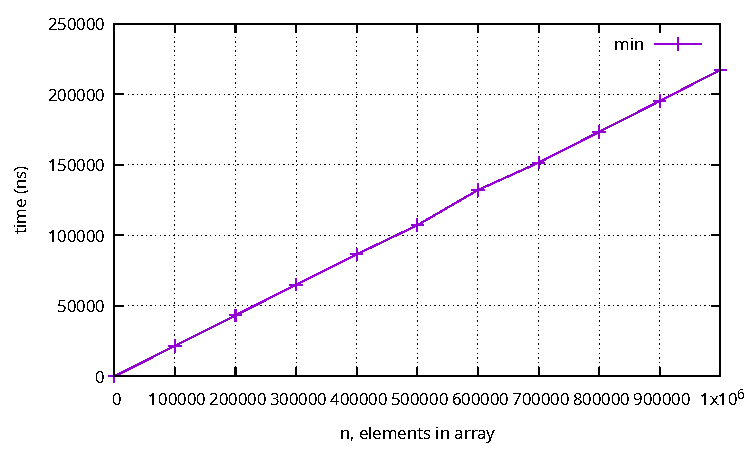
\includegraphics[scale=0.8]{graphs/plot_brute_unsorted.pdf}
		\caption{
			Graph showing the time it took to search for an item in an unsorted array with brute-force.
		}
	\end{figure}
	\par
	From looking at \textbf{Figure 1} we see this algorithm has a time complexity of roughly \(O(n)\).
	My measurements ended at an array containing 1,000,000 elements, for which it took around 0.22 milliseconds per search.

\section{Sorted Array}
	If we instead work with a sorted array our options become much more interesting.
	We can begin by doing a quick optimization that checks if the element we are comparing against is bigger than what we are looking for, and if so break.
	This works since all elements after will be even bigger than what we are looking for,
	which means it would be impossible for our element to exist further back in the array (if it is indeed correctly sorted).
	\begin{figure}[H]
		\centering
		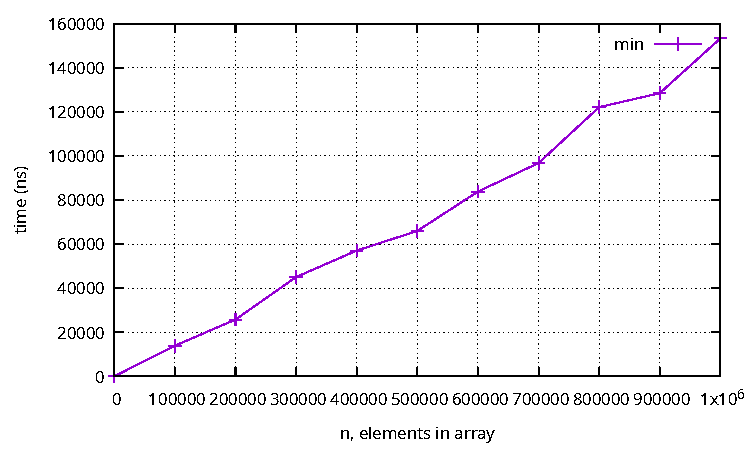
\includegraphics[scale=0.8]{graphs/plot_brute_sorted.pdf}
		\caption{
			Graph showing the time it took to search for an item in a sorted array with brute-force.
		}
	\end{figure}
	\par
	From looking at \textbf{Figure 2} we again spot a time complexity of \(O(n)\).
	This time, for an array containing 1,000,000 elements, it took around 0.15 milliseconds per search.
	This is roughly 27\% faster compared to the 0.22 milliseconds we measured earlier.

\section{Binary Search}
	Binary search is similar to what a human would do when looking up, for example, a word in a dictionary.
	If the word we are looking for starts with a 'T', it should be impossible for the word to be listed in any of the sections for letters that come before 'T'.
	Therefore, we can skip all of those which saves us a lot of precious time.
	We continue to apply this logic, jumping either backward or forward, until we have found the word we are looking for.
	For binary search to work correctly, the array MUST be sorted.
	\par
	In this part I will refer to what we are looking for as \textit{x}, since I feel that makes it easier to follow along.
	When it comes to numbers our best bet is to always start in the middle of the elements we have to choose from.
	That gives equal odds for \textit{x} to be on either side.
	In the beginning, the range of elements to choose from span the entire array,
	but as we continue to search the range will become smaller and smaller until we either find \textit{x} or run out of elements to compare against.
	We compare the number in the middle with \textit{x}, for which there are 3 possible outcomes:
	\begin{itemize}[label=\textbullet]
		\item If the numbers are equal, we have found a match!
		\item If \textit{x} is less than the middle value, we change our range to be the first half of our last range.
		\item If \textit{x} is bigger than the middle value we change our range to be the second half of our last range.
	\end{itemize}
	\begin{figure}[H]
		\centering
		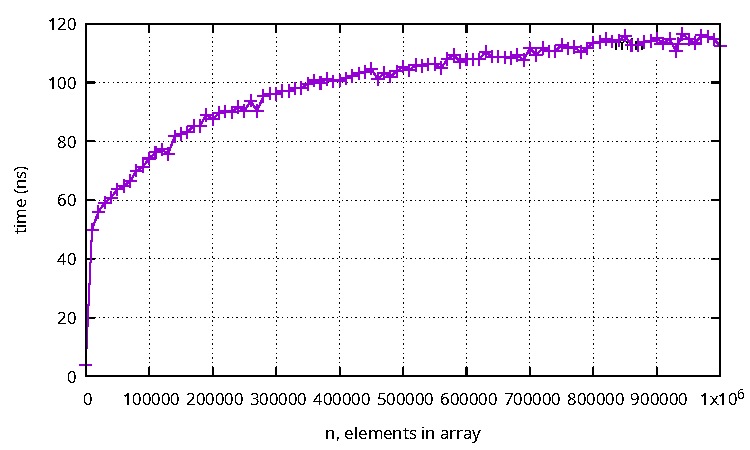
\includegraphics[scale=0.8]{graphs/plot_binary.pdf}
		\caption{
			Graph showing the time it took to search for an item in a sorted array with binary search.
		}
	\end{figure}
	\par
	As we can see in the \textbf{Figure 3} the time complexity of the binary search seems to follow \(O(\log n)\).
	The time I measured for 1,000,000 elements was now down to around 113 ns, which is orders of magnitude faster than the previous two algorithms.
	Our graph should roughly follow the following formula:
	\[t(n) = c \cdot \log n\]
	Here, \(t(n)\) represents the time taken for a given size \(n\), and it should be proportional to a logarithmic function scaled by a constant \(c\).
	This means we can calculate a rough estimate of \(c\) via the following:
	\[c = \frac{t(n)}{\log n}\]
	For \(n = 1{,}000{,}000\) and a logarithmic scale of base 2, I got \(c \approx 5.6\).
	With this I estimated that it would take around 146 ns for 64,000,000 elements.
	However, when I ran the benchmark I actually got that it took around 571 ns.
	This is most likely due cache misses, branch misspredictions, and other hardware related factors which get more significant as the array grows in size.
	Since binary search involves jumping around to different parts of the array,
	it is less cache-friendly compared to algorithms that access memory sequentially, for example.

\section{Recursion}
	Lastly, we were asked also implement binary search recursively.
	Recursive programming could make an implementation easier to follow along (or not).
	In this case I actually felt it was a bit easier to implement than the non-recursive approach.
	However, a big downside of recursive method calls is that the program stack has to be used extensively for storing said calls.
	\begin{figure}[H]
		\centering
		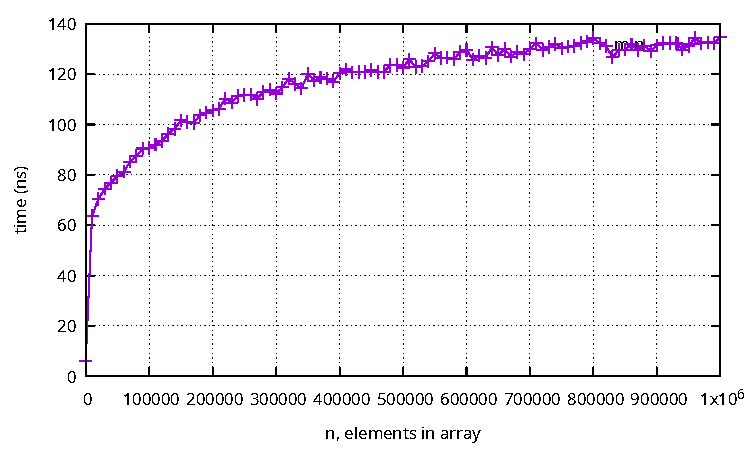
\includegraphics[scale=0.8]{graphs/plot_binary_recursive.pdf}
		\caption{
			Graph showing the time it took to search for an item in a sorted array with binary search (implemented with recursion).
		}
	\end{figure}
	\par
	In \textbf{Figure 4} we see the performance hit of using recursion in this case.
	It is however not that bad, since the time complexity has not changed, and the drop in performance was only around 20\%, but it is still important to take into consideration.

\section{Source Code}
	If anyone is interested, the source code for this project can be found over at:
	\url{https://github.com/neogulgul/ID1021/tree/main/searching}

\end{document}
